\section*{Trace 6: Symbolic Reflection in Wine Dataset}
\label{section:trace6_symbolic_reflection_wine}

\textit{This SRV trace extends the behavior established in Trace~5, further illustrating the symbolic dynamics of Definition~ through derivative visualization.}

\subsection*{1 Objective}
\label{subsection:trace6_objective}

Apply symbolic drift–reflection analysis to procedural data. This trace mirrors Trace 5 using the UCI Wine Quality dataset, evaluating residuals and sparsity under $L^p$ regression.

\subsection*{2 Validation Setup}
\label{subsection:trace6_validation_setup}

A linear model was trained on the UCI Wine Quality dataset under a sweep of $p \in \{1.0, 1.2, \ldots, 2.0\}$ norms. Metrics recorded:
\begin{itemize}
    \item \textbf{Residual Error:} Mean absolute error across $p$
    \item \textbf{Sparsity:} Number of near-zero coefficients (thresholded by magnitude)
\end{itemize}

\subsection*{3 Symbolic Responses and Figures}
\label{subsection:trace6_symbolic_responses_figures}

\begin{figure}[H]
\centering
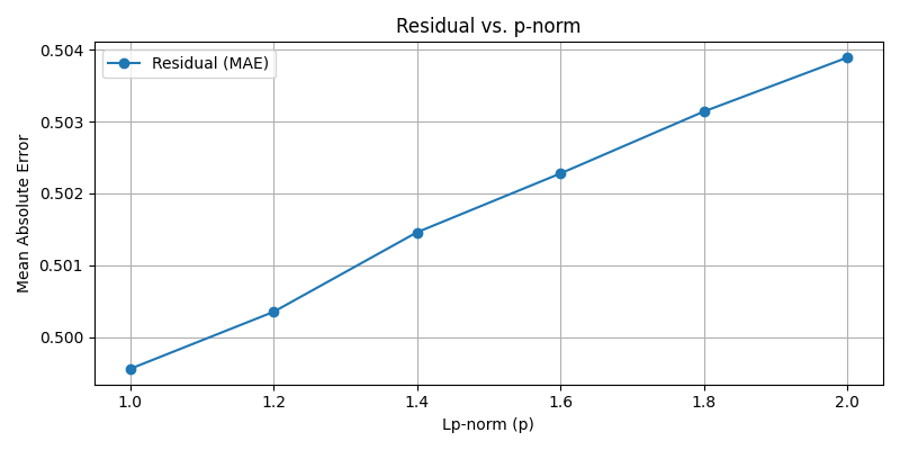
\includegraphics[width=0.85\textwidth]{srv_traces/6_residual_vs_p.png}
\caption{Residual MAE across Lp-norms on the Wine dataset}
\label{figure:trace6_residual_mae_wine}
\end{figure}

\begin{figure}[H]
\centering
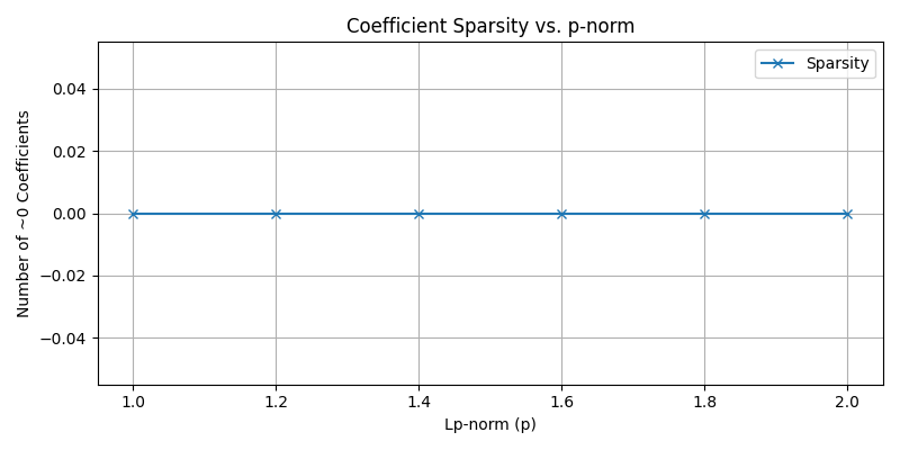
\includegraphics[width=0.85\textwidth]{srv_traces/6_sparsity_vs_p.png}
\caption{Sparsity vs. Lp-norm on Wine dataset}
\label{figure:trace6_sparsity_wine}
\end{figure}

\subsection*{4 Conclusion}
\label{subsection:trace6_conclusion}

The symbolic drift–reflection pattern observed in synthetic traces recurs within observer-bound real-world data. The Wine dataset exhibits smooth residual and sparsity gradients across $p$, supporting symbolic emergence beyond abstract simulation.

\subsection*{5 Theory Linkage}
\label{subsection:trace6_theory_linkage}

\begin{itemize}
    \item \textbf{Theorem 2.2:} Second Law of Symbolic Thermodynamics
    \item \textbf{Theorem 7.1:} Reflective Convergence to Stable Identity
    \item \textbf{Book IX Themes:} Emergence of symbolic viability under constraint
\end{itemize}
